
El conocimiento empírico se suele asociaciar a la ciencia y la técnica.
Aquí proponemos considerar a la vida como la principal fuente conocimiento empírico en tanto las diversas formas que ella adquiere en el curso de la evolución contiene información capaz de interectuar con el medio y sobrevivir.
Veremos que la complejidad actual de la vida es consecuencia de una serie de transiciones evolutivas en las que las entidades, que antes eran capaces de replicarse de forma independiente, luego de la transición sólo pueden replicarse como parte de una unidad mayor (e.g. células eucariotas, organizmos multicelular, especies sociales).
En el capítulo \ref{ch:iso} mostraremos que la naturaleza multiplicativa de los procesos de selección son la causa que genera sistemáticamente esta emergencia irreversible de la cooperación y la especialización.

% Parrafo

Segundo, revisaremos cómo la transición cultural de nuestra especie, que primero nos permitió dejar de estar en peligro de extinción y luego nos permitió ser capaces de ocupar en pocos años todos los nichos ecológicos de la tierra.
Veremos que la cultura es una propiedad poblacional que se ve influenciada por la estructura de la red de intercambios, que la integración y el aislamiento afectan los procesos de evolución cultural.%, como fue el caso de la involución cultural sufrida por Europa occidental durante la edad media y el extraordinario desarrollo ocurrido luego de su integración privilegiada al sistema mundo gracias a la plata americana.
Para estudiar cómo cambian las habilidades de las personas en el tiempo, en el capítulo \ref{ch:ttt} implementamos el modelo estado del arte en la industria del video juego, el cual nos permitió estudiar factores de aprendizaje social que afectan la habilidad esperada por simple experiencia individual, cómo el la formación de equipos (capítulo \ref{ch:team}) y la posición en de los individuos en red (capítulo \ref{ch:topo})

% Parrafo

Por último, revisamos el surgimiento de la ciencia moderna en su contexto histórico.
Examineremos cómo el criterio de autoridad feudal, reinterpretado como criterio de universalidad masculina blanca, sirvió de justificación para la aribitrariedad durante la era de genocidios culturales y ecológicos de la todavía vigente colonial-modernidad.
La masiva pérdida de diversidad cultural trajo como consecuencia la masiva pérdida de biodiversidad actual, una crisis ecológica sin precedentes.
A pesar de todos los avances, la ciencia metropolitana moderna no ha sido capaz de compensar la pérdida de los conocimientos milenarios acumulados por las comunidades autónomas locales.
Los sistemas culturales capaces de superviviencia a largo plazo desarrollaron de forma independiente tecnologías bien adaptados para la coexistencia intercultural y ecológica basada en cosmovisiones que, como la inferencia bayesiana, no solo permite sino que obliga a creer al mismo tiempo en hipótesis mutuamente contradictorias, A y no A.
En el capítulo \ref{ch:proba} definiremos revisaremos las reglas de la teoría de la probabildiad desde una perspectiva Bayesiana, la cual será la utilizada a lo largo de toda la tesis.

% Propondremos el concepto de honestidad, definido como maximización de la incertidumbre dada la evidencia, como principio intercultural de acuerdos intersubjetivos y por lo tanto como criterio de validez universal del conocimiento empírico cultural.
% Se hace necesario practicar la co-existencia inter-comunitaria, de modo de reactivar localmente los procesos de evolución cultural que le permitieron a nuestra especie adptarse a los diversos nichos ecológicos sin afectarlos en sus proceso vital, fuente real del conocimiento empírico.
%  

\section{Vida}

\en{In the last third of the history of the Universe, sometime around 4 billion years ago, a simple form of matter organization capable of self-replication appeared on Earth. }%
\es{En el último tercio de la historia del Universo, en algún momento hace aproximadamente 4000 millones de años, apareció en la tierra una forma de organización de la materia capaz de auto-replicarse. }%
%
\en{The growth of these lineages followed multiplicative and noisy processes: sequences of survival and reproduction rates. }%
\es{El crecimiento de estos linajes siguieron procesos multiplicativos y ruidosos: secuencias de probabilidades de supervivencia y reproducción. }%
%
\en{The errors produced during replication diversified the life forms, and the growth rates of the different strategies favored those better adapted to the environment. }%
\es{Los errores producidos durante la replicación diversificaron las formas de vida, y las tasas de crecimiento de las diferentes estrategias favorecieron a aquellas mejor adaptadas al ambiente. }%
%
\en{From that moment until now, life has acquired an extraordinary complexity, both in terms of cooperation and specialization. }%
\es{Desde aquel momento hasta ahora la vida adquirió una extraordinaria complejidad, tanto a nivel de cooperación como de especialización. }%
%
\begin{figure}[H]
    \centering
    \begin{subfigure}[b]{0.65\textwidth}
    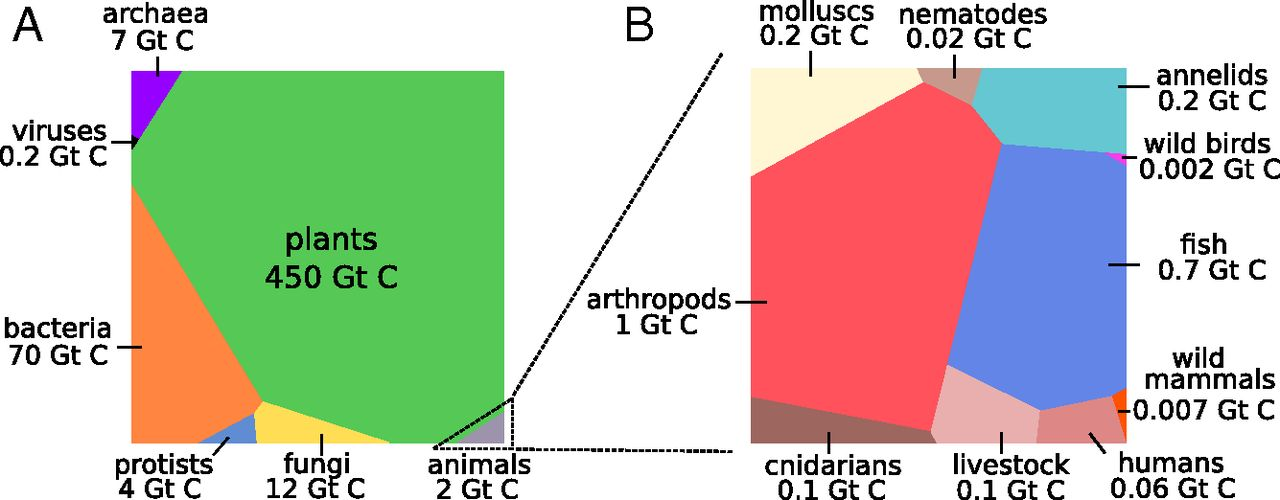
\includegraphics[width=\linewidth]{static/biomass.jpg}
    \end{subfigure}
    \caption{
    \en{Distribution of biomass on Earth estimated by Bar-On et al.~\cite{barOn2018-biomass}. }
	\es{Distribución de la biomasa en la Tierra estimada por Bar-On et al.~\cite{barOn2018-biomass}. }%
    }
    \label{fig:biomass}
\end{figure}
%
\en{The current complexity of life is the consequence of a series of evolutionary transitions in which entities capable of self-replication after the transition become part of higher level cooperative units~\cite{maynardSmith1995-majorTransitions, szathmary1995-evolutionaryTransitions, szathmary2015-evolutionaryTransitions}. }%
\es{La complejidad actual de la vida es consecuencia de una serie de transiciones evolutivas en las que entidades capaces de autoreplicación luego de la transición pasan a formar parte de unidades cooperativas de nivel superior~\cite{maynardSmith1995-majorTransitions, szathmary1995-evolutionaryTransitions, szathmary2015-evolutionaryTransitions}. }%
%
\en{Some of the paradigmatic transitions are: from prokaryotic to eukaryotic cells; from protozoa to animals, plants and fungi (cell differentiation and emergence of multicellular organisms); and from solitary individuals to societies. }%
\es{Algunas de las transiciones paradigmáticas son: de las células procariotas a las eucariotas; de los protozoa a los animales, plantas y hongos (diferenciación celular y emergencia de organismos multicelulares); y de los individuos solitarios a las sociedades. }%
%
\en{How to explain this permanent tendency of life in favor of cooperative and specialization? }%
\es{¿Cómo se explica esta tendencia permanente de la vida en favor de la cooperación y la especialización? }%
%``The transition must be explained in terms of inmmediate selection advantage to individual replicators'' szathmary1995-evolutionaryTransitions

% Parrafo

\en{In evolution it is said that the growth of a lineage over time, $\omega(t)$, is governed by a stochastic sequence of survival and reproduction rates $f(\cdot)$ dependent on a random environment $\Aa$, }
\es{En evolución se dice que el crecimiento de un linaje en el tiempo, $\omega(t)$, esta gobernado por una secuencias estocástica de tasas de supervivencia y reproducción $f(\cdot)$ dependientes de un ambiente aleatorio $\Aa$, }%
%
\begin{equation} \label{eq:modelo_exponencial}
\omega(T) = \prod_t^T f(\Aa(t)) \approx g^T
\end{equation}
%
\en{where $\Aa(t)$ represents the state of the environment at time $t$ and $g$ represents the characteristic growth rate when $T$ is sufficiently large. }%
\es{donde $\Aa(t)$ representa el estado del ambiente en el tiempo $t$ y $g$ representa la tasa de crecimiento caracterísitica cuando $T$ es suficientemente grande. }%
%
\en{For example, suppose nature flips a coin, if it comes up heads the population reproduces 50\% and if it comes up tails it survives 60\%. }%
\es{Por ejemplo, supongamos que la naturaleza lanza una moneda, si sale cara la población se reproduce 50\% y si sale seca sobrevive 60\%. }%
\begin{equation} \label{eq:estrategia_base}
f(\Aa) =
\begin{cases}
 1.5 & \Aa = \text{ \en{Head}\es{Cara} } \\
 0.6 & \Aa = \text{ \en{Tail}\es{Sello} }
\end{cases}
\end{equation}
%
\en{A similar example was proposed by Lewontin and Cohen (1969)~\cite{lewontin1969-randomlyVaryingEnvironment},  in which the population reproduces 70\% or survives 50\%. }%
\es{Un ejemplo similar fue anlizado por Lewontin y Cohen (1969)~\cite{lewontin1969-randomlyVaryingEnvironment}, en el que la población se reproduce 70\% o sobrevive 50\%. }%
%
\en{Different strategies $\Ee$ can be described with different functions $f_\Ee(\Aa)$. }%
\es{Diferentes estrategias $\Ee$ las podemos describr con diferentes funciones $f_\Ee(\Aa)$. }%
%
\en{According to the standard model of evolution, known as \emph{replicator dynamic} \cite{taylor1978-replicatorDynamic}, the change in the proportion of a strategy in the population, $x_\Ee$, is determined by its characteristic growth rate $g_\Ee$, }%
\es{Según el modelo estándar de evolución, conocido como \emph{replicator dynamic} \cite{taylor1978-replicatorDynamic}, el cambio de la proporción de una estrategia en la población, $x_\Ee$, está determinado por su tasa de crecimiento caracterísitica $g_\Ee$, }%
% schuster1983-replicatorDynamics, hofbauer2003-evolutionaryGameDynamics
%
\begin{equation} \label{eq:replicator_dynamic}  \tag{Replicator dynamic}
\hspace{3cm} x_\Ee^\prime = \frac{x_\Ee g_\Ee}{\sum_i x_i g_i}
\end{equation}
%
\en{where the denominator acts as a normalization constant. }%
\es{donde el denominador actúa como constante de normalización. }%
%
\en{But, what is the characteristic growth rate $g$? }%
\es{¿Cuál es la tasa de crecimiento característica $g$? }%
%
\en{Much of the evolutionary literature bases its analysis on populations of infinite size and considers that the correct estimate is obtained by the expected value, $g^t = \langle \omega \rangle_t$. }%
\es{Buena parte de la literatura en evolución basa su análisis en poblaciones de tamaño infinito y considera que la estimación correcta se obtiene mediante el valor esperado, $g^t = \langle \omega \rangle_t$. }%
%
\begin{equation}
\langle \omega \rangle_t = \sum_{\omega \in \Omega_t} \omega \cdot  P(\omega)
\end{equation}
%
\en{Where $\Omega_t$ is the set of all possible resource trajectories at time $t$, and $P(\omega)$ is the probability that the resource state $\omega$ occurs. }%
\es{Donde $\Omega_t$ es el conjunto de todas las posibles trayectorias de los recursos en el tiempo $t$, y $P(\omega)$ es la la probabilidad de que ocurra el estado de los recursos $\omega$. }%
% 
\en{In the coin example, the expected value in the first two time steps is, }%
\es{En el ejemplo de la moneda, el valor esperado en los dos primeros pasos temporales es, }%
%
\begin{equation}
\begin{split}
\langle \omega_e \rangle_1 & = 1.5 \cdot \frac{1}{2} + 0.6 \cdot  \frac{1}{2} = 1.05 \\ 
\langle \omega_e \rangle_2 &=  1.5^2 \cdot \frac{1}{4} + 2 (0.6 \cdot 1.5 \cdot \frac{1}{4} ) + 0.6^2 \cdot \frac{1}{4}= 1.05^2
\end{split}
\end{equation}
%
\en{That is, the estimated growth rate according to the expected value is $5\%$ for each time step, $\langle \omega \rangle_t = 1.05^t$. }%
\es{Es decir, la tasa de crecimiento estimada según el valor esperado es de $5\%$ por cada paso temporal, $\langle \omega \rangle_t = 1.05^t$. }%
%
\en{And indeed that is what happens with the average of several individual trajectories, $\omega(t)$. }%
\es{Y efectivamente eso es lo que ocurre con el promedio de varias trayectoria individuales, $\omega(t)$. }%
%
\begin{figure}[H]
    \centering
    \begin{subfigure}[b]{0.45\textwidth}
    \includegraphics[width=\linewidth]{figures/pdf/ergodicity_expectedValue.pdf}
    \end{subfigure}
    \caption{
    \en{Average of individual resources over time for different population sizes, in log scale. }%
    \es{Promedio de los recursos individuales en el tiempo para diferentes tamaños de la población, en escala logarítimica. }%
    %
    \en{As we increase the size of the population, the average approaches the expected value of $1.05^t$. }%
    \es{A medida que aumentamos el tamaño de la población, el promedio se acerca al valor esperado $\langle \omega \rangle_t = 1.05^t$. }%
    }
    \label{fig:ergodicity_expectedValue}
\end{figure}
%
\en{However, the expected value does not represent what happens to the agents over time. }%
\es{Sin embargo, el valor esperado no representa lo que le ocurre a los agentes en el tiempo. }%
%
\en{Individually, all the trajectories lose in the long term at a rate close to 5\%. }%
\es{Individualmente, todas las trayectorias pierden a largo plazo a una tasa cercana al 5\%. }%
%
\en{The trajectories observed in figure \ref{fig:ergodicity_individual_trayectories} are variable, but the longer we observe the system the smoother these lines become (figure \ref{fig:ergodicity_individual_trayectories_longrun}). }%
\es{Las trayectorias observadas en la figura \ref{fig:ergodicity_individual_trayectories} son variables, pero cuanto más tiempo observemos el sistema más suave se vuelven esas líneas (figura \ref{fig:ergodicity_individual_trayectories_longrun}). }%
%
\begin{figure}[H]
    \centering
    \begin{subfigure}[b]{0.45\textwidth}
    \includegraphics[width=\linewidth]{figures/pdf/ergodicity_individual_trayectories.pdf}
    \caption{}
    \label{fig:ergodicity_individual_trayectories}
    \end{subfigure}
    \begin{subfigure}[b]{0.45\textwidth}
    \includegraphics[width=\linewidth]{figures/pdf/ergodicity_individual_trayectories_longrun.pdf}
    \caption{}
    \label{fig:ergodicity_individual_trayectories_longrun}
    \end{subfigure}
    \caption{
    \en{The black line represents the expected value. }%
    \es{La recta negra representan el valor esperado. }%
    %
    \en{Figure \ref{fig:ergodicity_individual_trayectories}: size of individual resources over time, $ \log(\omega(t))$. }%
    \es{Figura \ref{fig:ergodicity_individual_trayectories}: tamaño de los recursos individuales en el tiempo, $ \log(\omega(t))$. }%
    %
    \en{Figure \ref{fig:ergodicity_individual_trayectories_longrun}: given enough time, all individual trajectories stick to the blue line. }% 
    \es{Figura \ref{fig:ergodicity_individual_trayectories_longrun}: con suficiente tiempo todas las trayectorias individuales se pegan a la recta azul. }% 
    }
    \label{fig:cpr_individual}
\end{figure}
%La relación entre el valor esperado y lo que le ocurre a los agentes individuales en el tiempo es un problema bien conocido en mecánica estadística.
\en{When the individual trajectories can be described by the expected value of the system states, then the process is said to be ergodic~\cite{peters2019-ergodicityEconomics}. }%
\es{Cuando lo que le ocurre a los agentes individuales en el tiempo puede describirse mediante el valor esperado de los estados del sistema, luego se dice que el proceso es ergódico~\cite{peters2019-ergodicityEconomics}. }%
%
\en{However, the conditions are very restrictive, and are not fulfilled in the case of multiplicative processes. }%
\es{Sin embargo, las condiciones para que esto se cumpla son muy restrictivas y no se satisfacen en el caso de los procesos multiplicativos. }%
%
\en{To compute the growth rate $g$, we first express the product as follows, }%
\es{Para calcular la tasa de crecimiento $g$, primero expresaramos la productoria de la siguiente manera, }%
%
\begin{equation}
\omega(T) = \prod^T_{t=1} f(\Aa(t)) = f(\text{\en{head}\es{cara}})^{n_1} f(\text{\en{tail}\es{sello}})^{n_2}
\end{equation}
%
\en{where $n_1$ and $n_2$ represents the number of occurrences of $f(\text{\en{head}\es{cara}})$ and $f(\text{\en{tail}\es{sello}})$, with $n_1 + n_2 = T$. }%
\es{donde $n_1$ y $n_2$ representa la cantidad de ocurrencias de $f(\text{cara})$ y $f(\text{seca})$, con $n_1 + n_2 = T$. }%
%
\en{In the limit, $T \rightarrow \infty$ all individual trajectories will be determined by the same growth rate $g$. }%
\es{En el límite, $T \rightarrow \infty$ todas las trayectorias individuales estarán determinadas por la misma tasa de crecimiento $g$. }%
%
\begin{equation} \label{eq:geometric_mean}
\begin{split}
\lim_{T \rightarrow \infty} \omega_e(T) & = {g}^T \\
\left( \lim_{T \rightarrow \infty} \omega_e(T) \right)^{1/T} & =  {g} \\
\lim_{T \rightarrow \infty} f(\text{cara})^{n_1/T} f(\text{seca})^{n_2/T} & 
 \end{split}
\end{equation}
%
\en{Where the frequencies $\frac{n_1}{T}$ and $\frac{n_2}{T}$ in the limit $T \rightarrow \infty$ are equal to the probabilities of the environmental states $p$. }%
\es{Donde las frecuencias $\frac{n_1}{T}$ y $\frac{n_2}{T}$ en el límite $T \rightarrow \infty$ son iguales a las probabilidades de los estados ambientales $p$. }%
%
\en{Therefore, the growth rate is, }%
\es{Por lo tanto, la tasa de crecimiento es, }%
%
\begin{equation}
g = (1.5 \cdot 0.6)^{1/2} \approx 0.95
\end{equation}
%
\en{This formula, which allows computing the long-term growth rate of individual trajectories, has previously been used in the evolution literature under the name \emph{geometric mean}~\cite{dempster1955-geometricMean}. }%
\es{Esta fórmula, que permite computar la tasa de crecimiento a largo plazo de las trayectorias individuales, ha sido usada previamente en la literatura de evolución bajo el nombre de \emph{media geométrica}~\cite{dempster1955-geometricMean}. }%
%
\en{The geometric mean is always less than the arithmetic mean (or expected value). }%
\es{La media geométrica es siempre es menor a la media aritmética (o valor esperado). }%
%
\en{This is because in multiplicative processes the physical impacts of losses are usually stronger than those of gains. }%
\es{Esto se debe a que en los procesos multiplicativos los impactos físicos de las pérdidas suelen ser más fuertes que los de las ganancias. }%
%
\en{In an extreme case, a single zero in the product is enough to generate an extinction. }%
\es{En un caso extremo, un único cero en la productoria alcanza para generar su extinción. }%

% Decimos que un proceso es ergódico si se cumple que,
% \begin{equation}
%  \underbrace{\lim_{T \mapsto \infty} \frac{1}{T} \sum_{t=1}^T \omega(t)}_{\text{Media temporal}}  = \underbrace{\sum_{\omega} \omega \cdot p(\omega)}_{\text{Media de estados}}
% \end{equation}
% 

\en{As a consequence of the non-ergodicity of multiplicative processes, fluctuations have a negative effect on individual growth rates. }%
\es{Como consecuencia de la no-ergodicidad de los procesos multiplicativos, las fluctuaciones tienen un efecto negativo en las tasas de crecimiento individuales. }%
%
%Parafraseando a Den Boer~\cite{denBoer1968-spreadingRisk}, la  supervivencia de una población depende de la distribución del riesgo dentro de la población y entre las poblaciones de diferentes especies.
\en{Yaari-Solomon~\cite{yaari2010-cooperationEvolution} and Peters-Adamou~\cite{peters-cooperation2019.03.04} (hereinafter Yaari and Peters) study the consequences that the following cooperative strategy has on the agents' growth rate. }%
\es{Yaari-Solomon~\cite{yaari2010-cooperationEvolution} and Peters-Adamou~\cite{peters-cooperation2019.03.04} (de aquí en adelante Yaari y Peters) estudian las consecuencias que la siguiente estrategia cooperativa tiene sobre la tasa de crecimiento de los agentes. }%
%
\begin{figure}[H]
\centering
\scalebox{0.75}{
\tikz{

    \node[latent, minimum size=2cm ] (x1_0) {$\omega_1(t)$} ;
    \node[latent, below=of x1_0, minimum size=2cm ] (x2_0) {$\omega_2(t)$} ;

    \node[latent, right=of x1_0, minimum size=3cm ] (x1_0g) {$ \omega_1(t)\cdot f(\Aa_1(t))$} ;
    \node[latent, right=of x2_0, minimum size=1.8cm, xshift=0.6cm , align=left] (x2_0g) {$\omega_2(t)\cdot$\\$f(\Aa_2(t))$} ;
    
    \node[latent, right=of x1_0g, minimum size=3.8cm, yshift=-1.33cm, align=right] (x_0) {$\omega_1(t)\cdot f(\Aa_1(t))$\\$+\omega_2(t)\cdot f(\Aa_2(t))$ } ;
    
    \node[const, above=of x_0] (nx_0) {$\overbrace{\text{Pool}\hspace{2.5cm}\text{Share}}^{\text{\normalsize Coopera\en{tion}\es{ci\'on}}}$} ;
    
    \node[latent, right=of x1_0g, minimum size=2.5cm,  xshift=4.5cm] (x1_1) {$\omega_1(t+1)$ } ;
    \node[latent, below=of x1_1, minimum size=2.5cm, yshift=0.7cm] (x2_1) {$\omega_2(t+1)$ } ;
    
    \edge {x1_0} {x1_0g};
    \edge {x2_0} {x2_0g};
    \edge {x1_0g,x2_0g} {x_0};
    \edge {x_0} {x1_1,x2_1};
    
}
}
\caption{
\en{The agents start with the same initial resources, update them independently according to the equation \ref{eq:estrategia_base}, and finally redistribute it in equal parts. }%
\es{Los agentes comienzan con los mismos recursos iniciales, los actualizan independientemente de acuerdo con la ecuación \ref{eq:estrategia_base}, y finalmente lo redistribuyen en partes iguales. }%
}
\label{fig:protocolo}
\end{figure}
%
\en{In Figure \ref{fig:ergodicity_cooperation} we show the trajectory of an agent in a cooperating group of size 33. }%
\es{En la figura \ref{fig:ergodicity_cooperation} mostramos la trayectoria de un agente en un grupo cooperador de tamaño 33. }%
%
\begin{figure}[ht!]
    \centering
    \begin{subfigure}[b]{0.45\textwidth}
    \includegraphics[width=\linewidth]{figures/pdf/ergodicity_cooperation.pdf}
    \end{subfigure}
    \caption{
    \en{The resources of an individual in a cooperative group of size 33 (green line) approaches the arithmetic mean (the black line below the green line).
    As a visual reference we show the geometric mean that drives the growth rate of individuals (blue line). }%
    \es{Los recursos de un individuo en un grupo cooperativo de tamaño 33 (recta verde) se aproxima a la media aritmética (la recta negra debajo de la recta verde).
    Como referencia visual mostramos la media geométrica que gobierna la tasa de crecimiento de los individuos (recta azul). }%
    }
    \label{fig:ergodicity_cooperation}
\end{figure}
%
\en{Fully cooperative groups reduce their fluctuations, generating an increase in the growth rate of all their members. }%
\es{Grupos enteramente cooperadoras reducen sus fluctuaciones, generando un aumento en la tasa de crecimiento de todos sus miembros. }%
% 
% \en{Individuals in fully cooperative groups achieve growth rates equivalent to the average of system states, which in non-ergodic systems is always higher than individual growth rates. }%
% \es{Los individuos de los grupos enteramente cooperadoras logran acceder a tasas de crecimiento equivalentes al promedio de estados del sistema, que en los sistemas no-ergódicos es siempre superior que la tasas de crecimiento individual. }%
%
\en{Peters-Amadou~\cite{peters-cooperation2019.03.04} believe that such increase in the growth rate is sufficient argument to demonstrate the evolutionary advantage of cooperation. }%
\es{Peters-Amadou~\cite{peters-cooperation2019.03.04} consideran que el aumento de la tasa de crecimiento es argumento suficiente para demostrar la ventaja evolutiva de la cooperación. }%
%
\en{However, they do not consider the problem of defection, who say ``our cooperators are unable to break the cooperative pact''. }%
\es{Sin embargo ellos no consideran el problema de la deserción, quienes dicen ``our cooperators are unable to break the cooperative pact''. }%
%
\en{This does not seem to be a minor problem, considering the temptation to stop contributing to the common fund while continuing to receive its benefits. }%
\es{No parece ser un problema menor, teniendo en cuenta la tentación de dejar de aportar al fondo común mientras se siguen recibiendo sus beneficios. }%

% Parrafo
\begin{framed}
\en{To explain why major evolutionary transitions are so common in the history of life we need to find the causes that systematically generate the irreversible emergence of cooperation and specialization. }%
\es{Para explicar por qué las grandes transiciones evolutivas son tan comunes en la historia de la vida necesitamos encontrar las causas que sistemáticamente generan la emergencia irreversible de la cooperación y la especialización. }%
%
\en{In \textbf{chapter \ref{ch:iso}} we show that, even if we consider \emph{unconditionally} cooperative individuals who generate a common good that can be exploited by defecting individuals without receiving some kind of punishment in return (e.g. end of cooperation), cooperative individuals are favored by multilevel selection. }%
\es{En el \textbf{capítulo \ref{ch:iso}} mostramos que, incluso si consideramos individuos \emph{incondicionalmente} cooperadores que generan un bien común que puede ser explotado por individuos desertores sin que reciban a cambio algún tipo de castigo (e.g fin de la cooperación), los individuos cooperadoras se ven favorecidos mediante selección multinivel. }%
%
\en{In addition, we show that as soon as cooperation emerges, an advantage in favor of specialist strategies appears. }%
\es{Además, mostramos que apenas surge la cooperación, aparece una ventaja a favor de las estrategias especialistas. }%
%
\en{Since the specialist strategies are individually poorly adapted to the environment, an irreversibility of the evolutionary transition is created. }%
\es{Como la estrategias especialistas están individualmente mal adaptadas al ambiente, se crea una irreversbilidad de la transiciones evolutivas. }%

% Parrafo

\en{The reason why an advantage in favor of cooperation and specialization arises in our simple causal model is due to the multiplicative (non-ergodic) nature of probabilitic and evolutionary selection process. }%
\es{El motivo por el cual surge una ventaja a favor de la cooperación y la especialización en este simple modelo causal se debe a la naturaleza multiplicativa (no-ergódica) los procesos de selección probabilístico y evolutivo. }%
%

\end{framed}

% 
% En el último tercio de la historia del Universo, en algún momento hace aproximadamente 4500 millones de años, apareció en la tierra una forma de organización de la materia capaz de auto-replicarse.
% El crecimiento de estos linajes siguieron procesos multiplicativos y ruidosos: secuencias de probabilidades de supervivencia y reproducción.
% Los errores producidos durante la replicación diversificaron las formas de organización de la materia, y las diferentes tazas de superviencia favorecieron a aquellas mejor adaptadas al medio.
% Las diversas formas que fue adquiriendo la vida representa información que es capaz de interectuar con el medio y sobrevivir.
% En este sentido, la vida puede ser vista conocimiento empírico y la evolución como un sistema natural de validación de la información empírica.
% 
% % Parrafo
% 
% La complejidad actual de la vida~\cite{barOn2018-biomass} es consecuencia de una serie de transiciones evolutivas~\cite{maynardSmith1995-majorTransitions} en las que las entidades, que antes eran capaces de replicarse de forma independiente, luego de la transición pasan a replicarse sólo como partes de una unidad mayor.
% La tabla~\ref{tab:transitions} enumera algunas de las principales transiciones ocurridas en la historia evolutiva de la vida.
% \begin{table}[ht!] \centering
%     \begin{tabular}{l}
%         \hline
%         \es{De moléculas a poblaciones de moléculas}
%         \\%        
%         \es{De células procariotas a eucariotas}
%         \\%
%         \es{De clones asexuales a poblaciones sexuales}
%         \\%
%         \es{De entidades unicelulares a multicelulares}
%         \\%
%         \es{De individuos a sociedades}
%         \\
%         \hline
%     \end{tabular}
%     \caption{
%     \es{Algunas de la principales transiciones evolutivas}
%     }
%     \label{tab:transitions}
% \end{table}
% Los saltos en los niveles de complejidad traen consigo la aparición de formas de ``división social del trabajo'' al interior de las poblaciones (e.g. diferenciación funcional de las células en organismos multicelulares), y cambios en el almacenamiento y transmisión de información (e.g. los sistemas de información cultural en las especies sociales).
% 
% % Parrafo
% 
% Hasta hace poco se consideró una verdad establecida que la cooperación requería algún tipo de comportamiento altruista para evolucionar.
% Esta conclusión suponía implícitamente que los procesos evolutivos eran ergódicos.
% Decimos que un proceso es ergódico si la media de los estados temporales del sistema (o de una transformación $f$ de ellos) es igual a la media de todos los posibles estados,
% \begin{equation}
%  \underbrace{\lim_{T \mapsto \infty} \int_0^T f(\omega(t)) \diff t}_{\text{Media temporal}}  = \underbrace{\int_{\Omega} f(\omega)p(\omega) \diff\omega}_{\text{Media de estados}}
% \end{equation}
% donde $\omega \in \Omega$ representa los estados del sistema, $\omega(t)$ el estado del sistema obtenido aleatoriamente en el tiempo $t$ y $p(\cdot)$ la distribución de probabilidad de los estados.
% Esta distinción es importante porque cuando un sistema es no-ergódicos, lo que le ocurre a los agentes individuales en el tiempo no coincide con la esperado según los posibles estados del sistema~\cite{peters2019-ergodicityEconomics}.
% 
% % Parrafo
% 
% El proceso multiplicativo al que está sujeto la vida es no-ergódico.
% Fundamentalmente porque los impactos de las pérdidas son más fuertes que los de las ganancias.
% Con que haya un cero en la secuencia de probabilidades de supervivencia y reproducción, cualquier linaje está queda extinto para siempre.
% Dado que la varianza realmente importa, una forma eficaz de reducirla es compartir los riesgos~\cite{yaari2010-cooperationEvolution, peters2015-evolutionaryAdvantageOfCooperation}.
% Por este motivo, los procesos evolutivos ofrecen una ventaja física a favor de los comportamientos cooperativos y diversificados.
% Para entender el mecanismo, consideremos el siguiente ejemplo.
% La naturaleza lanza una moneda: si sale cara la riqueza crece un 50\%, si sale cruz la riqueza se reduce un 40\%.
% \begin{equation}
% \Delta x =
% \begin{cases}
%  +0.5x & \text{ \en{Head}\es{Cara} } \\
%  -0.4x & \text{ \en{Tail}\es{Seca} }
% \end{cases}
% \end{equation}
% ¿Qué es lo que le ocurre a un agente en cada paso?
% Si el agente comienza con una riqueza inicial de $100$, hay una probabiilidad de $0.5$ que termine con $150$ y una probabilidad de $0.5$ que termine con $60$.
% La media es $105 = 150\cdot0.5 + 60\cdot0.5$.
% Los agentes tendrán en promedio un cambio positivo de su riqueza de $\langle \Delta x \rangle = 5\%$.
% Basados en este criterio, las corrientes principales de la teoría económica y de la teoría de toma de decisiones suponen que un agente racional debe tomar la apuesta.
% %Los experimentos con humanos muestra que las personas rechaza sistemáticamente esta tipo de apuestas, por lo que .
% Sin embargo, lo que le ocurre a los agentes individuales en el tiempo es muy diferente: a largo plazo todos pierden.
% En la figura \ref{fig:simple_gamble} mostramos esas trayectorias individuales en el tiempo.
% % 
% % \begin{figure}[ht!]
% %     \centering
% %     \begin{subfigure}[b]{0.45\textwidth}
% %     \includegraphics[width=\linewidth]{figures/pdf/cpr_individual.pdf}
% %     \caption{}
% %     \label{fig:simple_gamble}
% %     \end{subfigure}
% %     \begin{subfigure}[b]{0.45\textwidth}
% %     \includegraphics[width=\linewidth]{figures/pdf/cpr_cooperation.pdf}
% %     \caption{}
% %     \label{fig:simple_gamble_incesto}
% %     \end{subfigure}
% %     \caption{
% %     Riqueza de los agentes en el tiempo: en la figura \ref{fig:simple_gamble} los agentes juegan individualmente, en la figura \ref{fig:simple_gamble_incesto} algunos agentes comparten su riqueza en cada iteración.
% %     }
% %     \label{fig:gamble}
% % \end{figure}
% 
% Por el contrario, cuando los agentes comparten su riqueza todos se benefician a largo plazo.
% Las curvas verdes de la figura \ref{fig:simple_gamble_incesto} representa a una población de 100 agentes que luego de cada iteración colocan su riqueza individual en un fondo común que es dividido en partes iguales.
% La estrategia cooperativa le permite obtener lo que inicialmente esperábamos observar en cada paso, 5\% de ganancia por iteración.
% 
% % Parrafo
% 
% % \begin{equation}
% %     \bordermatrix{ & C & 1D & 99D  \cr
% %       C & 1.05 & 1.04 & -\infty \cr
% %       D & 2 &  & 0.95  } 
% % \end{equation}
% 
% El mecanismo solidario parece a primera vista fácil de ser explotado por agentes individualistas que desertan de aportar su riqueza al fondo común pero que siguen aprovechando de la distribución de la riqueza del resto.
% Las curvas azules y roja de la figura \ref{fig:simple_gamble_incesto} son las trayectorias de una población de 100 agentes con un único agente desertor en su interior, y con 10 agentes desertores respectivamente.
% Si bien los comportamientos desertores obtienen una ventaja relativa respecto de los miembros cooperadores de su propia población, desertar en una población enteramente cooperadora implica una reducción de la riqueza incluso para quien deserta.
% Los desertores, al afectar la riqueza de aquellos sobre los que se beneficia, se ven también perjudicados a largo plazo.
% %No hay agentes altruistas.
% 
% % Parrafo
% 
% Para entender por qué la mutua cooperación es la estrategia óptima, veamos en detalle un ejemplo.
% \begin{table}[ht!] \centering
%     \begin{tabular}{|l|c|c|c|c|c|c|c|}
%      \hline
%         {\small Agentes} & {\small \en{Wealth}\es{Riqueza}} & {\small \en{Growth}\es{Aumento}} & {\small \en{Wealth}\es{Riqueza}} & {\small \en{Sharing}\es{Reparto}} & {\small \en{Growth}\es{Aumento}} & {\small \en{Wealth}\es{Riqueza}} & {\small \en{Sharing}\es{Reparto}} \\ \hline \hline
%         A no-coop& $1$ & $\Delta +0.5$ & $1.5$ & $1.5$ & $\Delta -0.4$ & $0.9$ & $\bm{0.9}$ \\ \hline
%         B no-coop & $1$ & $\Delta -0.4$ & $0.6$ & $0.6$ & $\Delta +0.5$ & $0.9$ & $\bm{0.9}$ \\ \hline\hline
%         A coop & $1$ & $\Delta +0.5$ & $1.5$ & $1.05$ & $\Delta -0.4$ & $0.63$ & $\bm{1.1}$ \\ \hline
%         B coop & $1$ & $\Delta -0.4$ & $0.6$ & $1.05$ & $\Delta +0.5$ & $1.58$ & $\bm{1.1}$\\ \hline
%     \end{tabular}
%     \caption{
%     Evolución de la riqueza en procesos multiplicativos para agentes que no cooperan (primera dos filas) y agentes que sí cooperan (segundas dos filas).
%     }
%     \label{tab:gamble}
% \end{table}
% En la tabla \ref{tab:gamble} podemos ver cómo se modifica la riqueza individual de dos agentes en el tiempo cuando no cooperan y cuando cooperan.
% Ambas personas comienzan con la misma riqueza y modifican su riqueza del mismo modo pero en distito orden: en la primer paso la riqueza del agentes A aumenta y la del agente B se reduce, y viceversa.
% Los agentes que no dividen su riqueza en la columna ``Reparto'' terminan perdiendo 10\% de su riqueza inicial, mientras que los agentes que sí la dividen finalizan con 10\% más de su riqueza inicial.
% Mediante la cooperación los agentes tienen acceso a los diversos estados del sistema, lo que hace que sus trayectorias temporales $\overline{x}$ se aproximen al valor esperado $\langle x \rangle$.
% 
% % Parrafo
% 
% La naturaleza multiplicativa de los procesos evolutivos, i.e. la secuencia de probabilidades de superviencia y reproducción, ofrecen una ventaja física en favor de la agregación cooperativa de las entidades individuales.
% Para el surgimiento de nuestra especie se requirieron varias trasiciones evolutivas de este tipo.
% Lo que hace a los humanos especialmente inteligentes hoy no es sólo su capacidad cognitiva individual, sino fundamentalmente la capacidad de adquirir información cultural heredada.
% Otros animales también son capaces de crear herramientas, transmitir conocimiento entre generaciones y desarrollar tradiciones culturales.
% Sin embargo, el nivel de complejidad y diversificación de la acumulación cultura humana no tiene comparación.
% La ciencia es uno de esos sistemas de información cultural que emergieron como una propiedad poblacional a través del tiempo.
% 
% % Parrafo
% 
% Al mismo tiempo, la evolución favorece las formas de vida más ``económicas'' y por lo tanto más simples.
% El éxito adaptativo basado en el sistema de información cultural se ve relativizado cuando consideramos que nuestra especie representa sólo el 0.01\% de la biomasa actual de la tierra.
% En la figura~\ref{fig:biomass} vemos estimaciones recientes~\ref{barOn2018} de la distribución de la biomasa en el planeta tierra.
% \begin{figure}[ht!]
%     \centering
%     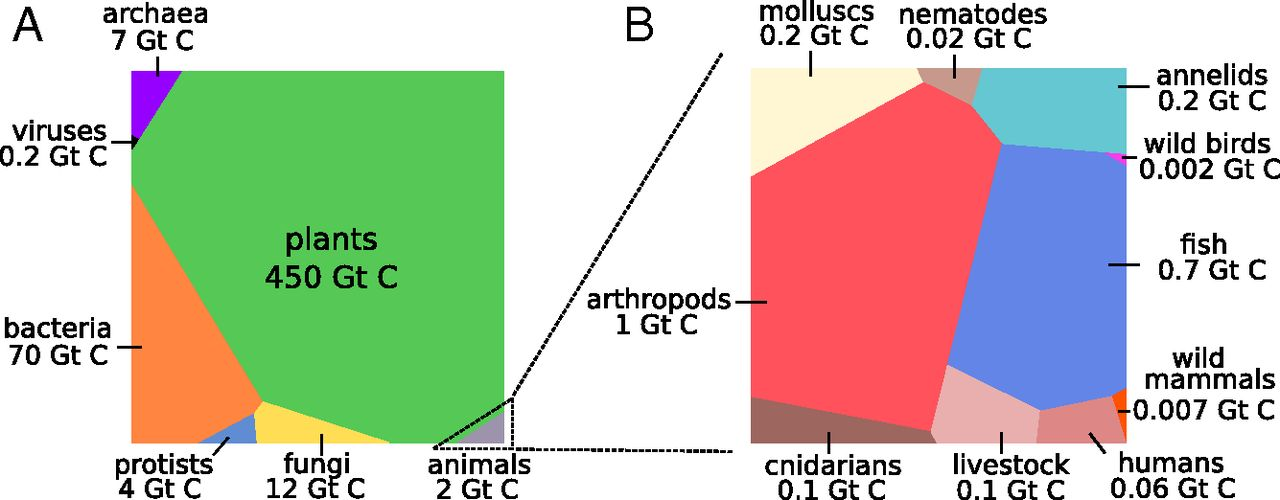
\includegraphics[width=0.7\linewidth]{static/biomass}
%     \caption{
%     \es{Distribución de la biomasa en el planeta tierra. }%
%     }
%     \label{fig:biomass}
% \end{figure}
% En el gráfico de la izquierda podemos ver que la plantas y las bacterias representan el 95\% de la biomasa de la tierra.
% En este sentido, la capacidad de adaptación de la información que estas especies almacenan en su sistema genético es varios órdenes de magnitud superior al alcanzado por los seres humanos mediante sus complejos sistemas de información cultural.

\section{Cultura}

La especial integraci\'on de los procesos biol\'ogicos, cognitivos y sociales que permiten a los humanos desarrollar culturas complejas se debió a una coevolución genético-cultural que se desencadenó por el desarrollo previo de la crianza cooperativa~\cite{hrdy2020-emotionallyModern}.
La forma en la que estos homininos organizaron la crianza produjo un ambiente que favoreció la selección de jóvenes capaces de monitorear y comprender las intenciones de los demás, y de atraer la atención de sus cuidadores de modo de compartir sus propias necesidades.
Antes del surgimiento de los humanos \emph{anatómicamente} modernos (masa cerebral actual) y de los humanos \emph{conductualmente} modernos (lenguaje), surgió en África una linaje \emph{emocionalmente} moderno~\cite{hrdy2020-emotionallyModern}.

% Parrafo

La empatía fue la que permitió el desarrollo del Homo sapiens: la comprensión mutua, la imitación, el lenguaje y finalmente la cultura.
Esta costosa habilidad cognitiva es especialmente eficiente para la adquisición de tradiciones complejas.
Lo que antes debía ser redescubierto una y otra vez mediante costosa experiencia individual, ahora podía ser transmitido a la siguiente generación.
La capacidad de adquirir comportamientos basados en la experiencia de otros sin tener que re-construirlos cada vez por prueba y error conduce un proceso de evolución y acumulativa cultural que permite a las poblaciones humanas adaptarse rápidamente ante cambios bruscos en el ambiente o migraciones a nuevos entornos.

% Parrafo

El surgimiento de la cultura produjo cambios radicales para nuestra especie.
Antes de la transición cultural, estuvimos en grave peligro de extinción, lo que se evidencia en la baja diversidad del genoma humano.
Luego de la transición cultural, en pocos años nuestra especie ocupó todos los nichos ecológicos de la tierra como ningún otro vertebrado terrestre lo había logrado antes.
Esta proeza se logró mediante los sistemas culturales y tecnológico desarrollados por sociedades cazadores-recolectores.
Caminando salimos de África, ocupamos Asia, y de allí Oceanía y las Américas (las flechas del mapa~\ref{fig:agricultura}).
La información transgeneracional fue la que le permitió a estas sociedades simples adaptarse rápidamente a los nuevos desafíos ecológicos.

% Parrafo

El cambio climático ocurrido al inicio del Holoceno (hace 12000 años) propició el desarrollo de la agricultura, que surgió de manera indendiente en los seis grandes sistemas geográficos de la tierra: en la región central de África subsahariana, en Asia occidental, en Asia oriental, en Oceanía norte, en América del norte y en América del sur (las puntos rojos del mapa~\ref{fig:agricultura}).
\begin{figure}[ht!]
    \centering
    \begin{subfigure}[b]{0.6\textwidth}
     \includegraphics[width=\textwidth]{figures/agricultura.pdf}
     \caption{Poblamiento de la tierra y agricultura}
     \label{fig:agricultura}
    \end{subfigure}
%     \begin{subfigure}[b]{0.40\textwidth}
%     \includegraphics[width=\textwidth]{static/polynesia.png} 
%     \caption{Poblamiento del océano Pacífico}
%     \label{fig:polynesia}
%     \end{subfigure}
    \caption{
    El mapa de la figura~\ref{fig:agricultura} es una proyección políedrica de la tierra que conserva los tamaños relativos de los continentes.
    Las felchas indican el poblamiento, desde África a Asia, y de Asia hacia Oceanía y América.
    Los puntos rojos indican surgimiento independiente de agricultura.
    El mapa de la figura~\ref{fig:polynesia}, desarrollado por Thorsby~\cite{thorsby2016-polynesiaAmerica}, muestra el poblamiento de la Polynesia y los contactos con Ámerica evidenciados en el material genéticos. }%
    \label{fig:poblamiento}
\end{figure}
Alrededor de estos puntos se desarrollaron los principales centros poblacionales de la humanidad.
El aumento de la población promovió, a su vez, el desarrollo de nuevas innovaciones tecnológicas y científicas, como la escritura, la matem\'aticas, las ingenier\'ias, la astronomía, las ciencias políticas, entre otras.
Durante el año 1400 el mundo florecía de sociedades "prósperas"~\cite{dussel2004-sistemaMundo}: Aztecas en Ámerica del norte, Incas en Ámerica del sur, Tongas en el Pacífico, Bantúes en África sub-sahariana, los Árabes e Indios en Asia occidental y Chinos en Asia oriental, por mencionar algunos.

% Parrafo

El desarrollo tecnológico de todas estas sociedades fue extraordinario. 
El imperio de Tonga ocupaba hace siglos todo el oc\'eano Pac\'ifico (figura~\ref{fig:polynesia}) con sorprendentes tecnologías de navegación que le habían permitido tener intercambios con América, que se evidencian en el componente genético de los pueblos de la Polynesia~\cite{thorsby2016-polynesiaAmerica, ioannidis2020-polynesiaAmerica}.
En la región Inca se había desarrollado un sistema de intercambios basado en la reciprocidad de trabajo (minka, ayni y mita) que le permitía a las comunidades administrar eficientemente el uso de los bienes comunes y al Estado desarrollar la infrastructura en el vasto territorio montañoso~\cite{murra1978-organizacion}.
En la región Azteca se había desarrollado un extenso mercado regional con ciudades de hasta 300.000 habitantes, tres veces la ciudad de Venecia en esa misma época.%~\cite{www7.uc.cl}. %http://www7.uc.cl/sw_educ/historia/conquista/parte1/html/h54.html
El mundo \'Arabe comerciaba productos desde el Océano Pacífico, en las Filipinas, hasta el Oc\'eano Atl\'antico, en Marruecos, conectando las innovaciones culturales de distintos hemisferios del planeta~\cite{dussel2004-sistemaMundo}.
África siempre fue el continente más diverso cultural y genéticamente, pero quizás el centro más innovador en términos científicos y tecnologías haya sido la región de China~\cite{needham2004-generalConclusionsAndReflections}.


Gracias a estar ubicada en uno de los principales centros geográficos del planeta, China pudo emerger como el corazón del sistema de intercambios planetarios~\cite{pomeranz2000-divergence}.
Para el año 1400, China llevaba al menos 2000 de continuidad socio-pol\'itica, y 900 a\~nos de un estado meritocr\'atico en el cual sus miembros eran elegidos a trav\'es de concurso público (examen imperial).
Inventa el acero en el siglo segundo, el papel en el siglo sexto, la imprenta en el siglo octavo, el papel moneda en el noveno, la br\'ujula en el onceavo.
Desarrolla infraestructuras como el canal navegable \emph{Da Yunhe} de más de 1700 kilómetros para conectar la ciudad de Pekín con otras ciudades importantes, y la famosa muralla que en total superó los 20000km de longitud.
China ya era de hecho el principal proveedor comercial del resto del mundo.
No parecían necesitar nada más afuera de sus fronteras.
Luego de las exploraciones de Zheng He (1405-1433), el Gobierno Chino decide cerrarse fronteras adentro dándolas por finalizadas por completo.

% Parrafo

Así como la integración favorece los proceso de innovación y acumulación cultural, el asilamiento induce pérdidas masivas de información cultural.
Un ejemplo de aislamiento total bien documentado ocurre con la separación de Tasmania del continente Australiano por la subida del nivel del mar ocurrida a comienzos del Holonceno.
La evidencia arqueológica y etnohistórica indica que desde el principio del Holoceno las sociedades de Tasmania perdieron gran parte de su cultura tecnológica.
La principal hipótesis sugiere que la reducción del tamaño efectivo de la población (\emph{effective population size}) fue la causa más importante de estas pérdidas culturales~\cite{Henrich2004}.

\begin{figure}[ht!]     
  \centering 
  \begin{subfigure}[c]{0.45\textwidth}
    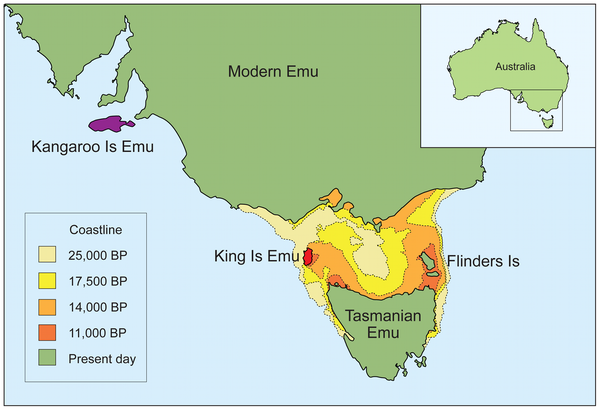
\includegraphics[width=\textwidth]{static/tasmania.png} 
    \caption{Tasmania}
    \label{fig:tasmania}
  \end{subfigure}
  \begin{subfigure}[c]{0.45\textwidth}
    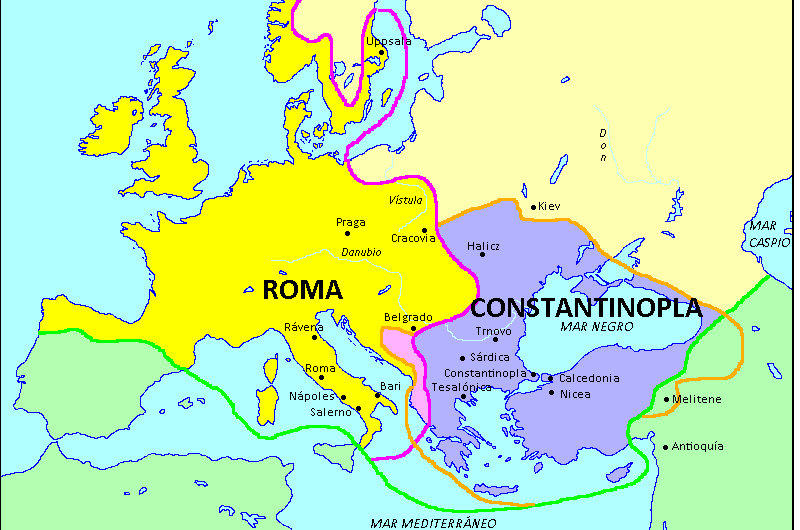
\includegraphics[width=\textwidth]{static/cisma.png} 
    \caption{Edad media}
    \label{fig:cisma}
  \end{subfigure}
  \caption{Aislamiento}
  \label{fig:aislamiento}
\end{figure}

Un caso de asilamiento parcial ocurre en Europa occidental.
Arrinconada ya en el lejano occidente por el fr\'io polar y la falta de tecnolog\'ias de navegaci\'on del Atlántico, Europa occidental comienza en el siglo octavo a quedar paulatinamente aislada del ``sistema mundo'' por la expansión Árabe al sur y por la serie cismas con el Imperio Bizantino al Oeste~\cite{Dussel}.
Esa etapa de aislamiento coincide con el proceso de perdida masivas de información cultural y de degradación de las condiciones socio-económicas conocido como ``edad media'', un proceso que sólo ocurre en Europa occidental.

\begin{framed}
\en{Culture is a population phenomenon that emerges as a consequence of the interaction between individuals. }%
\es{Como la cultura es una fenómeno poblacional que se transmite a través de redes de intercambios. }%
%
\en{Even individual experience is a fundamental factor for human learning, our unique social learning ability allows us to acquire knowledge based on the behaviors of others. }%
\es{Si bien la experiencia individual es un factor fundamental para el aprendizaje humano, nuestra peculiar capacidad de aprendizaje social nos permite adquirir conocimiento basado en los comportamientos de los otros. }%
%
\en{\T }%
\es{Para estimar las habilidades de las personas implementamos el modelo estado del arte en la industria del video juego, el cual permite obtener buenas estimaciones iniciales y grantizar su comparabilidad histórica (\textbf{capítulo \ref{ch:ttt}}). }%
%
Esto nos permitió estudiar cómo los factores de aprendizaje social afectan la habilidad esperada por simple experiencia individual.
%
En el \textbf{capítulo \ref{ch:team}} pudimos observar, en un juego en línea que permite formar equipos de distinto tamaño, que la tendencia a jugar en equipo se asocia con una mejora de las habilidades a largo plazo, mientras que jugar lealmente con el mismo compañero acelera significativamente la adquisición de habilidades a corto plazo.
%
\en{In an other we were able to verify that, studying the evolution of individual centralities over time, that intermediate centralities are associated with better learning curves (\textbf{chapter \ref{ch:topo}}). }%
\es{En otro juego pudimos ver además, estudiando la evolución de las centralidades individuales en el tiempo, que las centralidades intermedias están asociadas a mejores curvas de aprendizaje (\textbf{capítulo \ref{ch:topo}}). }%

\end{framed}

\section{Ciencia colonial-moderna}

La periodización histórica \emph{antigüedad} - \emph{edad media} - \emph{modernidad}, que coloca a Europa occidental como centro de la historia universal, es hoy sentido común y sigue estando vigente incluso en la principales universidades del mundo, desde la Universidas de Buenos Aires a Harvard, tanto en universidades de África, el mundo Árabe, India y Asia.
¿Qui\'enes propusieron por primera vez tal periodizaci\'on?
Es a fines del siglo 18 que Hegel populariza esta nueva periodizaci\'on hist\'orica que proyecta a la europa occidental en la cultura griega y judeo-cristiana, ambos fenómenos de origen oriental, con pretensión de explicación histórico-mundial: ``La historia universal va del Oriente al Occidente, Europa es el centro absoluto de la historia universal'' dice Hegel en su \emph{Filosofía de la historia universal}.

% Parrafo

Varios argumentos demuestra que tal periodizaci\'on es objetivamente falsa.
Por ejemplo, la historia de la ciencia que se imparte en esas universidades suele comenzar con Grecia, y continúa sin escalas en el desarrollo de la ciencia europa moderna.
Sin embargo, las obras de Aristóteles y Platón fueron fue traducidas al Latín luego de 1500 años de existencia, en base a traducciones Árabes y no a sus originales Griegos.
Pero para demostrar que tal periodizaci\'on es objetivamente falsa alcanza con señalar que sólo hubo \emph{edad media} en un área equivalente al 2\% de la tierra firme del planeta.
Y ya hemos visto que durante los años en los cuales europa occidental vivía su etapa más oscura, el mundo florecía de civilizaciones prósperas.

% Parrafo

La paradoja que no puede responder la fábula eurocéntrica es cómo una sociedad sumida en un proceso de involución cultural único, como la sociedad feudal de la ``edad media'', pudo generar de repenten el proceso de desarrollo científico y técnico de la modernidad.
Desde Hegel hasta la fecha, las explicaciones eurocéntricas intentan explicar la proposperidad actual de occidente a través de una causa interna: la ``ética protestante'' de Max Weber~\cite{weber1905-eticaProtestante}, la ``mentalidad burguesa'' de José Luis Romero~\cite{romero1967-revolucionBurguesa}, o más recientemente el ``sistema de parentezco'' de Joseph Henrich~\cite{henrich2020-weirdest}.
Incluso John Needham, el británico que dedicó su vida a recopilar la monumental historia científica y técnica de China, reconoce que comenzó a estudiar el tema motivado por responder la pregunta de por qué sólo Europa occidental había logrado el avance científico.
\begin{quotation}
When I first formed the idea, about 1938, (...) I regarded the essential problem as that of why modern science had not developed in Chinese civilisation (or Indian or Islamic) but only in that of Europe~\cite{needham2004-generalConclusionsAndReflections}.%
\end{quotation}
Luego de 60 años de investigaciones, Needham se ve obligado inviertir la pregunta.
\begin{quotation}
Why, between the -1th century and the 15th century, was Chinese civilisation much \emph{more} efficient than occidental in gaining natural knowledge and in applying it to practical human needs?~\cite{needham2004-generalConclusionsAndReflections}
\end{quotation}

% Parrafo

Ninguna de las explicaciones eurocéntricas incorpora en su análisis la situación de aislamiento que sufre Europa occidental en la etapa previa ni la coincidencia de eventos que puso de repente a esta sociedad, sumida en la violencia interna, en una situación de privilegio mundial.
Todos los conocimientos que la sociedad feudal europea va incorporando del resto de comunidades del mundo durante la colonial-modernidad se les borra su verdadero origen histórico y se las enaltecen como surgimientos espontaneos internos.
Pero la realidad es otra.

% Parrafo

Producto de la pésima situación socio-económica de la ``edad media'', europa occidental intenta varias veces, sin éxito, recuperar la integración al sistema mundo por el oriente.
Si bien la sociedad feudal no pudo avanzar por el oriente, pudieron lentamente ganar algo de terreno en la provincia más occidental del mundo Árabe, Al-Andaluz hoy España.
Si no era posible recuperar el acceso al sistema mundo por tierra, la opción que quedaba era explorar los mares del este.
La tecnologías de navegación eran mejores afuera en China y en el imperio de Tonga.
Pero apenas Europa occidental logra navegar el Atlántico, comienza un masivo proceso migratorio, típico de toda sociedad sumida en un proceso de grave violencia interna.
El flujo migratorio europeo hacia américa comienza a finales del siglo 15 y termina recién a mediados del siglo 20.

% Parrafo 

Además de la buena predisposición con la que los exploradores reportan haber sido recibidos por los habitantes Americanos, la llegada de masiva de emigrantes feudales produjo una serie de pandemias en América que redujeron la población local en al menos un 66\% entre los años 1500 y el 1600~\cite{koch2019-europeanArrival}.
Un siglo antes, China hab\'ia incorporado la plata como monedad oficial, la que ya estaba siendo utilizada como moneda de cambio en todo el mundo Árabe~\cite{pomeranz2000-divergence, pomeranz2018-tradeCreated}.
En América del sur el Estado Incaico que estaba organizado en base a un sistema de intercamios reciproicitarios no monetarios, era una región montañosa rica en plata.
Cuando 1546 los exploradores descubren la montaña de plata de Potosí, en el centro del sistema estatal incaico, la Europa feudal queda inmediatamente en una posición de privilegio en todo el mundo afro-euro-asiático.

% Parrafo

%Mediante la captura del sistema administrativo incaico (golpe de estado) los impuestos que antes antes se destinaban al desarrollo de la infraestructura, comienza a ser utilizado para extraer la plata, un mineral sin interés por los nativos.
Sólo 25 años después de haber descubierto la montaña de plata de Potosí en 1546, y 80 años después de haber logrado navegar el Atlántico, la sociedad feudal logra romper en el mediterraneo el cerco que la tenía asilada del sistema mundo, en la batalla de lepanto.
La plata, que ya era reconocida como moneda oficial en todo el mundo eruo-asiático, colocó de repente a esta sociedad marginal en una situación de integración privilegiada al sistema mundo.
La plata de América fluye en todas las direcciones, principalmente en dirección a China, y se inicia un proceso rápido de acumulación cultural basado en las tecnologías extranjeras.
\begin{figure}[ht!]     
  \centering 
  \begin{subfigure}[b]{0.48\textwidth}
    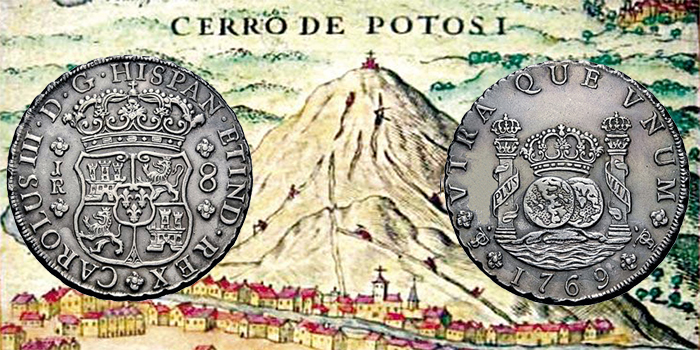
\includegraphics[width=\textwidth]{static/plata-potosi} 
    \caption{Plata}
    \label{fig:potosi}
  \end{subfigure}
   \ \ 
  \begin{subfigure}[b]{0.47\textwidth}
    \includegraphics[width=\textwidth]{figures/china.pdf} 
   \caption{Opio}
    \label{fig:china-pop}
  \end{subfigure}
  \caption{La plata y el opio como las llaves de la integración privilegiada de la Europa occidental en el sistema mundo.}
  \label{fig:integracion}
\end{figure}
Durante 250 años la plata americana sirvió para muchas cosas, pero principalmente para comprar productos chinos y financiar la primera industrialización británica con tecnología China.
Europa consumía productos asiáticos, pero exportaba muy poco a Asia.
El comercio internacional de opio comenzó a mediados del 1700 como respuesta a una crisis del comercio internacional europeo, especialmente británico.
El opio, un producto lujoso utilizado en China como medicina (raramente como estupefaciente), fue prohibida por los emperadores chinos en 1729, que por su abundancia hacía crecer lentamente la cantidad de adictos.
Las consecuencias fueron más graves cuando en 1818 se desarrolla una mezcla de opio más barata y potente.

% Parrafo

Mediante el narcotráfico Europa occidental consigue por primera vez, en el siglo 19, revertir el déficit comercial que históricamente tuvo con China.
El número de adictos llegó a ser lo suficientemente alarmante, y en 1839 China comete el error de declarar la guerra al narco-estado británico en su propio territorio.
Los resultados fueron terribles.
Los chinos no sólo no pudieron impedir el ingreso de la droga, perdieron también su autonomía arancelaria, el derecho a someter a los residentes extranjeros a la ley china.
Expuesta a su debilidad militar, China sufrió un siglo calamitoso de agresiones extranjeras, desorden interno y guerra civil, que produjo una caída de 1/5 de su población (figura~\ref{fig:china-pop}).

% Parrafo

Luego de la derrota de China por parte del narco-estado británico, se establece por pimera vez la hegemonía de Europa occidental en el sistema mundo y comienza un proceso de colonización en todo el mundo.%, que hasta el momento estaba limitado a América continental estaba limitada a puertos e islas.
En 1850 comienza la colonización de África continental y de los extensos territorios americanos que todavía seguían a manos de comunidades locales.
Comienza la era de los genoentocidios.
\begin{figure}[ht!]
    \centering
    \begin{subfigure}[b]{0.48\textwidth}
    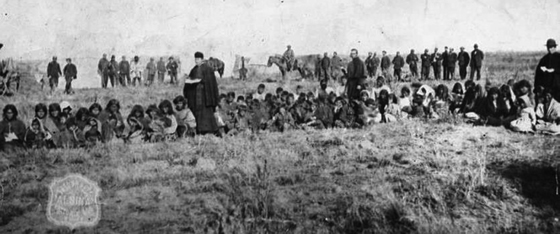
\includegraphics[width=\linewidth]{static/genocidio_patagonia}
    \caption{Genoetnocidios}
    \label{fig:genocidio_patagonia}
    \end{subfigure}
    \begin{subfigure}[b]{0.47\textwidth}
    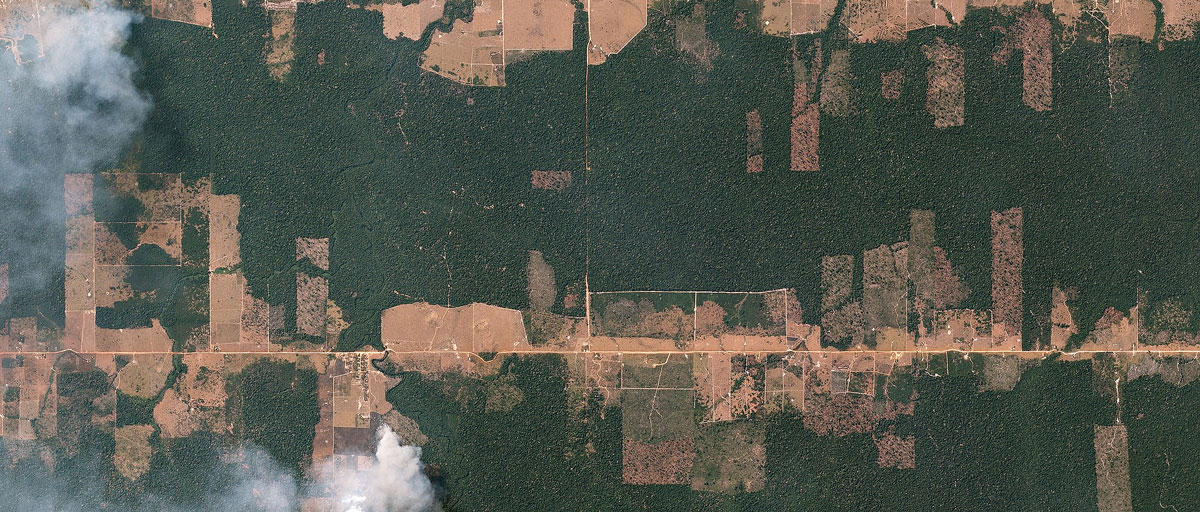
\includegraphics[width=\linewidth]{static/deforestation-brazil}
    \caption{Crisis ecológica}
    \label{fig:deforestation-brazil}
    \end{subfigure}
    \caption{
    La masiva pérdida de diversidad cultural trajo como consecuencia la masiva pérdida de biodiversidad actual, una crisis ecológica sin precedentes.
    }
    \label{fig:cultural-lose}
\end{figure}
En todas las partes del globo, los exploradores y etnógrafos fueron documentando la perdida de cultural debida al avance del frente colonial-moderno, estatal o privado, sobre las autonomías locales.
Es una nueva era de avances científicos y tecnológicos, pero por otro es la era de pérdida de diversidad cultural.
A pesar de todos los avances científicos, la ciencia metropolitana moderna no fue capaz de compensar la pérdida de los conocimientos milenarios acumulados por las comunidades autónomas locales.
La masiva pérdida de diversidad cultural trajo como consecuencia la masiva pérdida de biodiversidad actual, una crisis ecológica sin precedentes (figura~\ref{fig:deforestation-brazil}).

% 
% Europa occidental también estuvo constituida por este tipo de comunidades.
% Si bien el imperio romano eliminó una parte importante de este paisaje cultural, no alcanzó a eliminarlo por completo.
% Los ``bárbaros'' justamente eran comunidades autónomas establecidas en la parte norte de Europa occidental, que persistieron luego de la caída del imperio romano de occidente.
% Pero la ``edad media'' fue una anomalía en la historia de la humanidad.

% 
% % Parrafo


\subsection{Criterios de autoridad}

En la etapa de aislamiento comenzó a ganar terreno al interior de la sociedad feudal el criterio de autoridad (sexual, militar, académica, moral) como fundamento del ``saber auténtico''.
Durante la ``edad media'' las instituciones heredadas del imperio romano de occidente, en cabeza de la iglesia católica romana, comenzaron a competir con las comunidades indígenas locales y a producir una conjunto de novedosas tecnologías de colonización~\cite{zaffaroni2013-cuestionCriminal}. 
Una de las primeras y más importante fue la regulación de las relaciones comunitaria de reproducción, de forma más detallada que la propiedad.
Con esta acción se proscribió el rol político que las mujeres desempeñan en la administración del espacio doméstico comunitario, interviniendo en el funcionamiento de sus tecnologías de sociabilidad.
Se debilita así el arraigo comunitario, facilitando la captación de población desertora para actividades militares.
\begin{figure}[ht!]
    \centering
    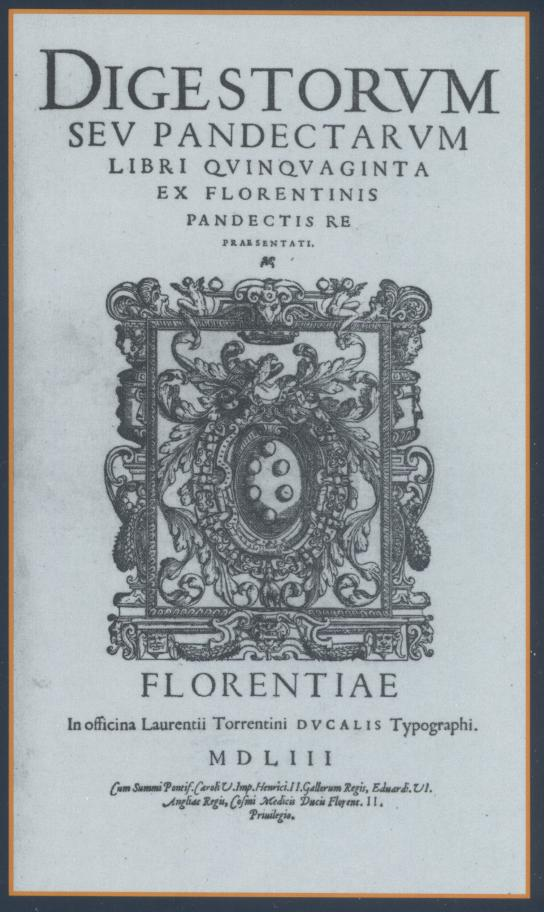
\includegraphics[width=0.15\linewidth]{static/digesto1553.jpg}
    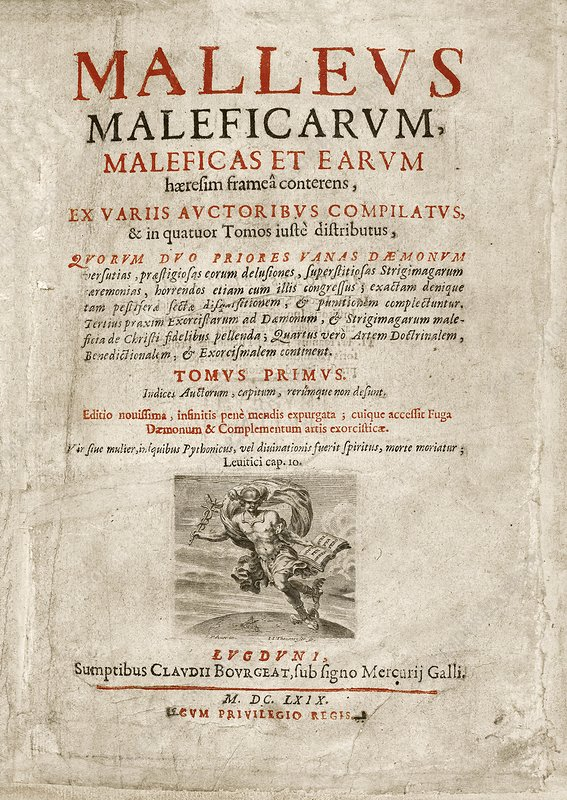
\includegraphics[width=0.178\linewidth]{static/malleus.jpeg}
    \caption{El criterio de autoridad como fundamento del ``saber auténtico'' y la guerra contra las mujeres como tecnología de colonización. %La proscripción de las tecnología de sociabilidad comunitaria, acción política del espacio doméstico administrada principalmente por las mujeres, debilita el arraigo comunitario facilitando la capatación de población desertora para actividades militares.
    }
    \label{fig:malleus}
\end{figure}
El poder punitivo se fue extendiendo y un nuevo sistema penal re-nació de los llamados \emph{libris terribilis} del Digesto, antiguas leyes romanas recolectadas por encargo del emperador Justiniano de Constantinopla pero re-interpretadas en occidente de modo de liberar al poder punitivo de todo límite.
En esta etapa, el sujeto masculino se torna modelo de lo humano y de todo cuanto sea dotado de politicidad, interés general y valor universal, y el espacio de las mujeres se transforma en margen y resto de la política.
La guerra contra las mujeres se formaliza definitivamente con la publicación del \emph{Malleus maleficarum} en 1484, que es el segundo best seller de la modernidad después de la Biblia durante los siguientes 200 años.

% Parrafo

Sólo después de que la sociedad feudal adquiere una posición de privilegio en el sistema mundo, comienza al interior de esta sociedad, ahora colonial-moderna, un nuevo debate sobre las fuentes de validación del conocimiento.
En esta etapa el criterio de experiencia personal comenzó ganar terreno como fundamento del ``saber auténtico'' sobre los criterios de autoridad.
Algunos lo entendieron la experiencia como ``evidencia intelectual'' (racionalistas) y otros como ``evidencia sensible'' (empiristas), dos grupos de exigencias que se consideraron al principio incompatibles entre sí: el de universalidad y necesariedad por un lado, y el de fuente y acreditación empírica por otro~\cite{samaja1999-epistemologiaYMetodologia}.
Sin embargo, de ambos lados existió un consenso de que el nuevo criterio, que servía para democratizar el conocimiento al interior de la sociedad feudal, estaba reservado para uso exclusivo de sus miembros varones.

% Parrafo

El argumento de la superioridad moral, que es utilizado durante toda la modernidad hasta el presente, lo desarrolla por primera vez Ginés de Sepúlveda cuatro años después del descubrimiento de la plata de Potosí, en 1550.
\begin{quotation}
 Será siempre justo y conforme al derecho natural que tales gentes [bárbaras] se sometan al imperio de príncipes y naciones más cultas y humanas, para que por sus virtudes y la prudencia de sus leyes, depongan la barbarie y se reduzcan a vida más humana y al culto de la virtud [...] Y si rechazan tal imperio se les puede imponer por medio de las armas, y tal guerra será justa según el derecho natural lo declara [...] En suma: es justo, conveniente y conforme a la ley natural que los varones probos, inteligentes, virtuosos y humanos dominen sobre todos los que no tienen estas cualidades~\cite{dussel2020-primerDebate}
\end{quotation}
Esta idea no se ve afectada por el argumento que propone Kant, conocido como el imperativo categórico, de que la validez del conocimiento radica en el reconocimiento mututo,
\begin{quotation}
Obra de tal modo que la máxima de tu voluntad pueda valer siempre al mismo tiempo como principio de una legislación universal~\cite{samaja1999-epistemologiaYMetodologia}% \cite{Kant2003:28}.
\end{quotation}
El criterio de autoridad feudal-colonial-moderno sin embargo continúa latente en el mismo Kant, quien no percibe una contradicción cuando unos parrafos más adelante él mismo considera que las razas americanas son incapaces de toda cultura y que las razas negras pueden ser educadas pero sólo como sirvientes y esclavos.
No hay contradicción porque el concepto de ``universalidad'' fedual-colonial-moderno nace limitado.
La sociedad colonial-moderna, y su ciencia, repite la estructura verticalista y punitivista de la sociedad feudal, ahora con alcance global.

% Parrafo

La Europa feudal no se había despertando del impacto de su invasión colonial cuando ya en 1514 Bartolomé de la Casas inicia desde América la advertencia de los efectos negativos de la integración basada en la dominación que promovían los primeros migrantes feudales~\cite{dussel2020-primerDebate}.
En su crítica Bartolomé:
a) refuta la pretensión de superioridad de la cultura occidental sobre las las culturas indígenas;
b) diferencia entre otorgar al otro (al indio) pretensión de verdad, sin renunciar a la pretensión de predicar a favor la propia cultura cristiana;
c) y demuestra la falsedad del argumento usado para justificar la intervención en las autonomías locales, basado en el supuesto ``remedio a las injusticias internas'', en tanto esas intervenciones producían peores efectos sobre las poblaciones intervenidas.

\subsection{Criterios de coexistencia}

El avance de la conquistual-modernidad estuvo (y está) motivado por una deficiencia social más que por una puramente material.
El mandato de exhibir públicamente alguna forma de poder para adquirir el estatus masculino hizo que los hombres derrotados se volvieran vulnerables al ejemplo de las masculinidades victoriosas coloniales.
En esta mutación histórica, las mujeres quedaron restringidas a la esfera íntima perdiendo su rol político en la administración del espacio doméstico y las tecnologías de sociabilidad.
Con el debilitamiento de los vínculos comunitarios, la cosmovisión individualista e instrumental logró introducirse cosificando todas las formas de vida.
Mujeres, extranjeros, animales y sistemas ecológicos completos participan sólo como objetos de los varones-blancos, estos últimos únicos sujetos con valor universal.

% Parrafo

El criterio de autoridad globalizado durante la colonial-modernidad como criterio de universalidad limitado a los varones blancos abrió la puerta a la aribitrariedad cultural y ecológica.
En efecto, luego de cinco siglos podemos ratificar sus efecto negativos: la masiva perdida de diversidad cultural primero y la masiva pérdida de biodiversidad en curso en la actualidad.
La intervención unilateral de un grupo de humanos sobre el sistema ecológico, reservorio del principal conocimiento empírico para la vida, es la analogía más acabada de la imposición de la mentira sobre la verdad.
Los conocimientos milenarios y sus instituciones adaptadas ecológicamente se pierden definitivamente en unas pocas generaciones y una crisis ecológica sin precedentes comienza.
  
% Parrafo

La experiencia acumulada a través de las generaciones por las más diversas comunidades del mundo condujo, de forma independiente, al desarrollo de tecnologías de reciprocidad, social y ecológica, sorprendentemente similares entre sí.
La misma naturaleza multiplicativa de los procesos evolutivos que había ofrecido una ventaja física para la agregación cooperativa de las formas de vida, favoreció también la aparición de instituciones culturales basadas en la reciprocidad.
Los pueblos bien adaptados para la coexistencia intercultural y ecológica practican cosmovisiones basadas en lógicas paraconsistentes que les permite creer en A y no A al mismo tiempo, pues la preferencia de una opción no se traduce en el rechazo de su complemento.
Recuperar las autonomías comunitarias se sustenta en el hecho práctico de que el único conocimiento cultural ecológicamente adaptado evoluciona sólo a través de la experiencia que acumulan los pueblos en el transcurso de su historia~\cite{segato2013-colonialidad}.

% Parrafo

Sus tecnologías de sociabilidad fueron fundamentales para su supervivencia durante la colonial-modernidad, pues a través de ellas lograron reducir las fluctuaciones individuales que hubieran desencadenado en el fin de su existencia como pueblo autónomo.
En todas ellas se pueden reconocer al menos dos mecanismos que cumplen la función de re-ciclar los v\'inculos interprersonales: los ritos festivos y los ritos coercitivos~\cite{segato2016-guerraContraLasMujeres}.
Los ritos coercitivos, presentes en todas las sociedades, no son otra cosa que ceremonias para la reactivación de flujos de intercambios rotos previamente por conflictos entre partes.
Están orientados el restablecimiento de los vínculos mediante los mecanismos de ``reparación'', ``conciliación'' y ``ayuda'' \cite{zaffaroni2013-cuestionCriminal}, haciendo uso de los tres tipos de intercambios posibles entre partes: dar ($\rightarrow$), intercambiar ($\leftrightarrow$) y recibir ($\leftarrow$).
La expulsión del agresor de la comunidad sólo se prevee en casos extremadamente excepcionales, pues el primer derecho de sus miembros es formar parte de la comunidad \cite{segato2016-guerraContraLasMujeres}.

% Parrafo

%Los sistemas penales del derecho romano instaurados por las Repúblicas independientes suspenden esta larga tradición de tecnologías de sociabilidad comunitaria, porque toma monopolio sobre el victimario y excluye a la víctima de la decisión.
%La identidad comunitaria y los ritos coercitivos tienden a darle estabilidad a los vínculos interpersonales, lo que favorece la estabilidad evolutiva de los comportamientos reciprocitarios en porblaciones que ya son reciprocitarias.

Estas cosmovisiones que permite creer en A y no A al mismo tiempo son también la base de las tecnologías de reciprocidad con la biocenosis que existen en todo el mundo, como son los ritos \emph{Canang sari} practicados en Bali o como los \emph{pachamámicos} practicados en América del sur.
\begin{figure}[ht!]
    \centering
    \begin{subfigure}[b]{0.45\textwidth}
    \centering
    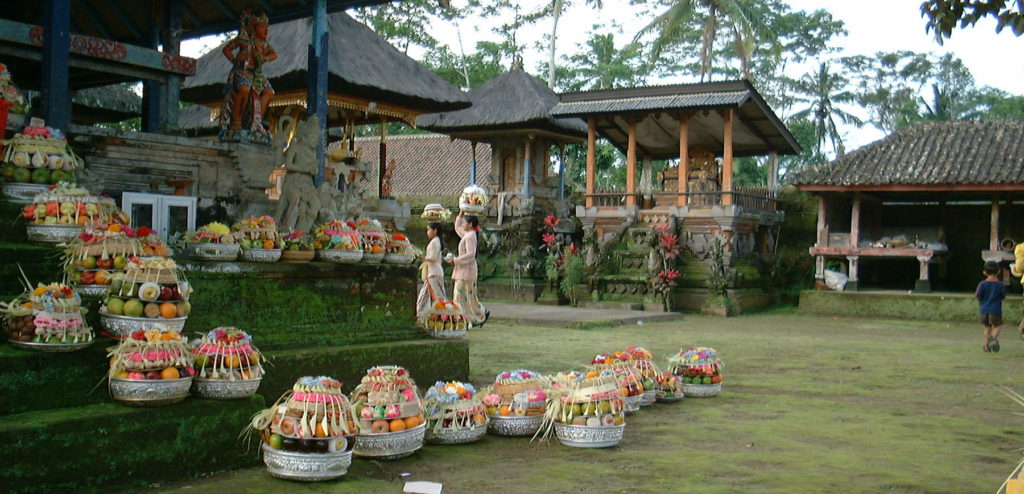
\includegraphics[width=\linewidth]{static/bali-offerings}
    \caption{Canang sari}
    \label{}
    \end{subfigure}
    \begin{subfigure}[b]{0.33\textwidth}
    \centering
    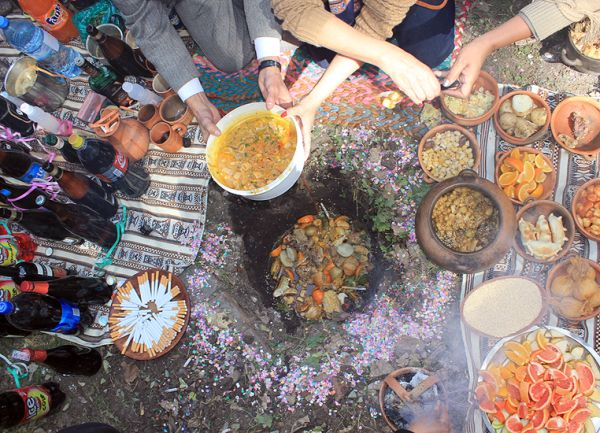
\includegraphics[width=\linewidth]{static/pachamama}
    \caption{Pachamama}
    \label{}
    \end{subfigure}
    \caption{Tecnologías de reciprocidad con la naturaleza.}
    \label{fig:mito}
\end{figure}
Estas cosmovisiones basadas en lógicas paraconsistentes obliga al ser humano, aunque se percibir en una posición de jerarquía respecto de otras especies, a respetar las otras formas de vida.
E incluso es la base de su estrategia de convivencia intercultural pues les permite creer al mismo tiempo en sus propios ritos y en la religión cristina que la sociedad colonial-moderna le quiso imponer como la única verdad.

% Parrafo

Los estudios comparados indican que las instituciones capaces de interactuar de forma estable con los sistemas ecológicos locales nunca fueron ni estatales ni privadas, siempre son de tipo comunitarias con un arraigo histórico local~\cite{ostrom2010,ostrom1990}.
En ellas se observa la presencia de las siguientes caracterísiticas:\vspace{-0.1cm}
\begin{description}\setlength\itemsep{-0.1cm}
 \item[1. Identidad comunitaria y territorial:] el reconocimiento de miembros y del sistema ecológico específico sobre el cual se ejerce la jurisdicción.
 \item[2. Normas acordes a la comunidad y el sistema ecológico:] Las normas son compatibles con las condiciones sociales y medioambientales locales.
 \item[3. Deliberación comunitaria:] La mayoría de los individuos involucrados en el sistema ecológico están autorizados a participar en la elaboración y modificación de sus normas.\setlength\itemsep{-0.1cm}
 \item[4. Conocimiento experto local:] La supervisión de los compartamientos de las personas el sistema ecológico está a cargo de los mismos miembros.\setlength\itemsep{-0.1cm}
 \item[5. Garantías de derechos comunitatrias:] Las sanciones son graduales, comienzan siendo muy bajas, y sólo raramente se decide la expulsión de la comunidad porque el primer derecho es formar parte de una comunidad.
 \item[6. Ritos festivos y coercitivos:] ceremonias de intercambio para el restablecimiento de los vínculos comunitarios mediante los mecanismos de ``reparación'', ``conciliación'' y ``ayuda''.
 \item[7. Autonomía comunitaria:] el reconocimiento de las comunidades vecinas a establecer sus propias normas.
 \item[8. Relaciones intercomunitarias] cuando un recurso de uso común está conectado a un sistema socioecológico más amplio, las actividades se organizan en múltiples capas anidadas.
\end{description}

% Parrafo

Para que las fluctuaciones que ahora están sufriendo otras especies no afecten a la nuestra de forma irreversible es necesario aplicar a escala planetaria las tecnologías de reciprocidad con la biocenosis que practican estas comunidades.
El criterio de coexistencia debe adquirir una universalidad que ni la propuesta parcial de Kant ni la cultura colonial-moderna ha sido capaz de alcanzar.
Es necesario que el imperativo categórico ``Obra de tal modo que la máxima de nuestra voluntad pueda valer siempre al mismo tiempo como principio de una legislación universal'' sea efectivo, reconociendo esta vez como sujetos con valor universal a todas las diversidades presentes: a las mujeres y su rol político que encabezan en el espacio comunitario, a las autonomías comunitarias locales, y el derechos de las otras especies y de la madre tierra toda de no ver interrumpido sus procesos sin justa causa: lo mínimo necesario para el buen vivir (\emph{suma kausay}).

\begin{framed}
En el capítulo \ref{ch:proba} definiremos un concepto de verdad para contextos de incertidumbre.
Reviaremos las dos soluciones principales a la contradicción vigentes en la actualidad, la naturalista (o frecuentista) y la epistémica (o Bayesiana).
Y finalmente, revisaremos las reglas de la teoría de la probabildiad desde una perspectiva Bayesiana, que será la utilizada a lo largo de toda la tesis.
\end{framed}

